\documentclass{standalone}

\usepackage{mathpazo}        % Loads Palatino + math support
\usepackage[utf8]{inputenc}
\usepackage{amsmath, amssymb, amsthm, amsfonts}
\usepackage{mathtools}       % For extra math tools
\usepackage{gensymb}         % Generic symbols
\usepackage{bm}              % Bold math symbols
\usepackage{enumitem}        % Better control over lists
\usepackage{geometry}        % Better margins
\usepackage[colorlinks=true, linkcolor=blue, urlcolor=blue, citecolor=blue]{hyperref}
\usepackage[tracking=true]{microtype}
\usepackage{xfrac}
\usepackage{tikz}            % Plots
\usepackage{tikz-3dplot}     % 3D plots
\usepackage{titlesec}        % Heading spacing control
\usepackage{siunitx}         % Alignment in matrices

\usepackage{tikz}
\usetikzlibrary{positioning,decorations.pathreplacing}

\begin{document}

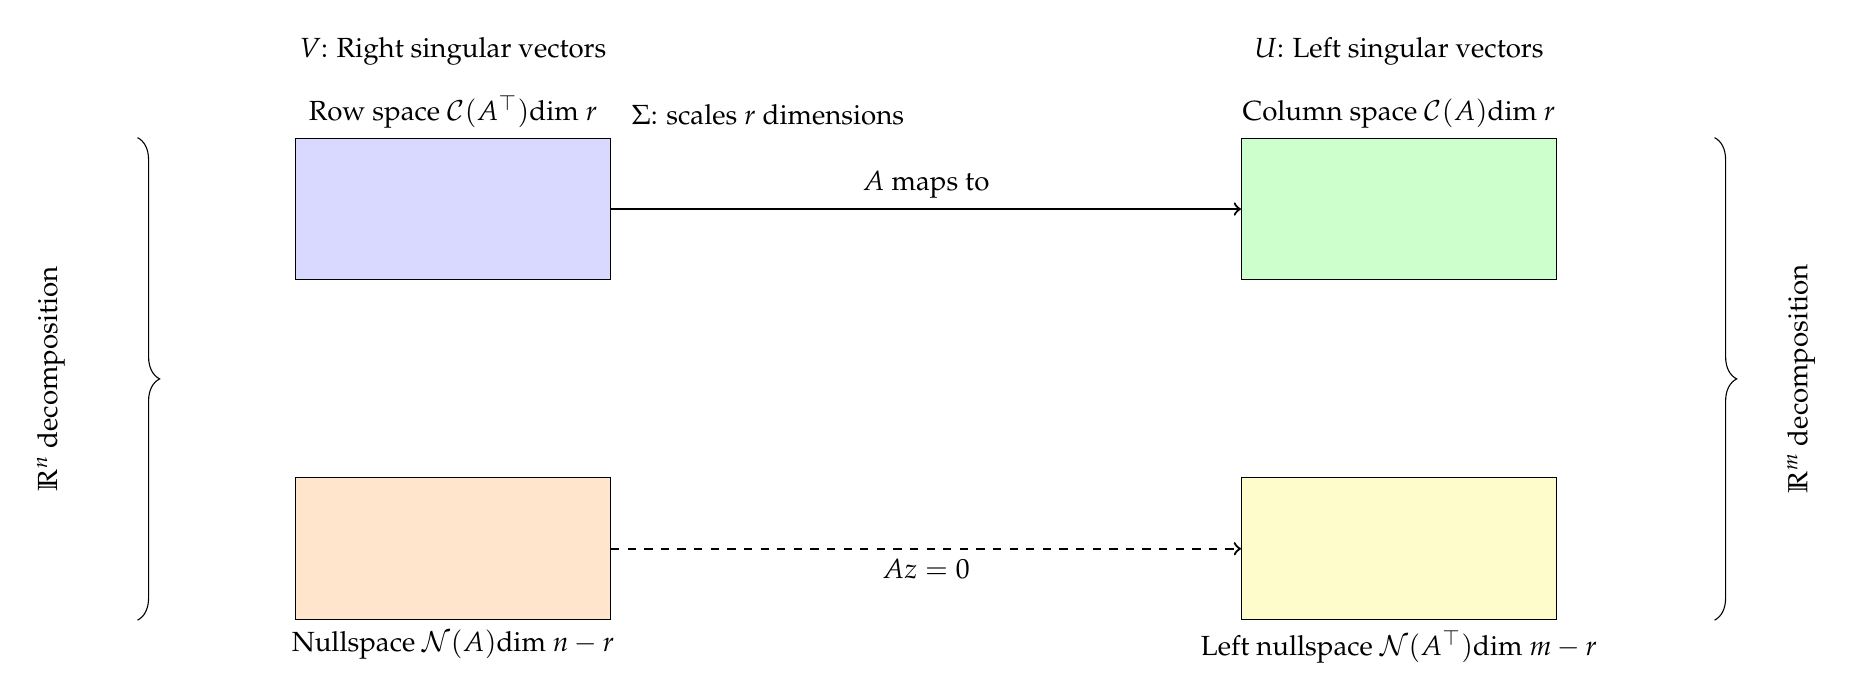
\begin{tikzpicture}[
        subspace/.style={draw, minimum width=4cm, minimum height=1.8cm, fill=blue!10},
        node distance=2.5cm
    ]

    % Left side: domain R^n
    \node[subspace, fill=blue!15, label=above:{Row space $\mathcal{C}(A^\top)$ \\ dim $r$}] (rowspace) at (0,0) {};
    \node[subspace, fill=orange!20, below=of rowspace, label=below:{Nullspace $\mathcal{N}(A)$ \\ dim $n-r$}] (nullspaceA) {};

    % Right side: codomain R^m
    \node[subspace, fill=green!20, right=8cm of rowspace, label=above:{Column space $\mathcal{C}(A)$ \\ dim $r$}] (colspace) {};
    \node[subspace, fill=yellow!20, below=of colspace, label=below:{Left nullspace $\mathcal{N}(A^\top)$ \\ dim $m-r$}] (nullspaceAT) {};

    % Braces for decompositions
    \draw[decorate,decoration={brace,amplitude=8pt}]
    ([xshift=-2cm]rowspace.north west) -- ([xshift=-2cm]nullspaceA.south west)
    node[midway,xshift=-1.1cm,rotate=90] {$\mathbb{R}^n$ decomposition};

    \draw[decorate,decoration={brace,amplitude=8pt}]
    ([xshift=2cm]colspace.north east) -- ([xshift=2cm]nullspaceAT.south east)
    node[midway,xshift=1.1cm,rotate=90] {$\mathbb{R}^m$ decomposition};

    % Arrows representing A
    \draw[->, thick] (rowspace.east) -- node[above] {$A$ maps to} (colspace.west);
    \draw[->, thick, dashed] (nullspaceA.east) -- node[below] {$Az = 0$} (nullspaceAT.west);

    % Annotations for SVD
    \node[above=0.8cm of rowspace] {$V$: Right singular vectors};
    \node[above=0.8cm of colspace] {$U$: Left singular vectors};
    \node at (4,1.2) {$\Sigma$: scales $r$ dimensions};

\end{tikzpicture}
\end{document}
